\documentclass[letterpaper]{article}
\usepackage{flairs}%aaai
\usepackage{times}
\usepackage{helvet}
\usepackage{courier}
\usepackage{graphicx}
\usepackage{setspace}
\usepackage{url}
\frenchspacing
\setlength{\pdfpagewidth}{8.5in}
\setlength{\pdfpageheight}{11in}
\pdfinfo{
/Title (Representation, Verification, and Visualization of Tarskian Interpretations for Typed First-order Logic)
/Author (Geoff Sutcliffe, Alexander Steen, Pascal Fontaine, Jack McKeown)} 

\setcounter{secnumdepth}{2}  

%----Making things more compact
\newcommand{\smalltt}[1]{\small \texttt{#1}}
\newenvironment{packed_itemize}{
\vspace*{-0.2em}
\begin{itemize}
\setlength{\partopsep}{0pt}
\setlength{\itemsep}{1pt}
\setlength{\parskip}{0pt}
\setlength{\parsep}{0pt}
}{\end{itemize}}
\newenvironment{packed_enumerate}{
\vspace*{-0.2em}
\begin{enumerate}
\setlength{\partopsep}{0pt}
\setlength{\itemsep}{1pt}
\setlength{\parskip}{0pt}
\setlength{\parsep}{0pt}
}{\end{enumerate}}
\renewcommand{\textfraction}{0.07}
\renewcommand{\topfraction}{0.9}
\renewcommand{\bottomfraction}{0.9}
\renewcommand{\floatpagefraction}{0.66}
\setlength{\floatsep}{2.0pt plus 2.0pt minus 2.0pt}
\setlength{\textfloatsep}{5.0pt plus 2.0pt minus 0.0pt}

%----For Alex's proof stuff
\usepackage{amsmath,amssymb,amsthm}
\newtheorem*{lemma}{Lemma}
\newtheorem*{theorem}{Theorem}
\newcommand{\true}{{\mathit{true}}}
\newcommand{\false}{{\mathit{false}}}

\begin{document}
% This file is an adoption of the style file for AAAI Press 
% proceedings, working notes, and technical reports.  This file is made 
% with minimal changes by explicit permission from AAAI.

\title{Representation, Verification, and Visualization of\\
Tarskian Interpretations for Typed First-order Logic}
\author{Anon One\\
Some where\\
Some place\\
Some country\\
\And
Anon Two\\
Some where\\
Some place\\
Some country\\
\And
Anon Three\\
Some where\\
Some place\\
Some country\\
\And
Anon Four\\
Some where\\
Some place\\
Some country}

\maketitle
\begin{abstract}
\begin{quote}
This paper describes a new format for representing Tarskian-style interpretations for formula in 
typed first-order logic, using the TPTP TF0 language.
It goes on to describe a technique and implemented tool for verifying models using this
representation, and a tool for visualizing interpretations.
The research contributes to the advancement of automated reasoning technology for model finding, 
which has several applications, including verification.
\end{quote}
\end{abstract}
%--------------------------------------------------------------------------------------------------
\section{Introduction}
\label{Introduction}

Automated Reasoning (AR), and Automated Theorem Proving (ATP) in particular, has focused largely 
on the task of proving theorems from axioms -- the derivation of conclusions that follow inevitably 
from known facts \cite{RV01-HAR}.
The axioms and conjecture to be proved (and hence become a theorem) are written in an 
appropriately expressive logic, and the proofs are often similarly written in logic \cite{SS+06}.
In this work typed first-order logic in the form of \cite{Wal83,Sch85,Coh87},
%  higher-order \cite{And86}, and some 
% on-classical \cite{Pri08} logics, 
whose expressive power is sufficient for a wide range of topics \cite{Sut17}, is used.
(This work is also applicable to untyped first-order logic,
% where terms have the type $\iota$ and formulae have the type $o$, 
and can also be generalized to higher-order logics.)

In the last two decades the converse task of disproving conjectures
% , i.e., proving that a 
% conjecture is not a theorem of the axioms, 
has become increasingly important.
This process depends on finding an {\em interpretation}, i.e., a structure that maps terms 
to domain elements and formulae to truth values.
An interpretation that maps a formula to {\em true} is a {\em model} of the formula.
A conjecture is disproved by finding an interpretation that is a model of the axioms, but 
maps the conjecture to {\em false}.
A salient application area that harnesses this form of ATP is verification \cite{DKW08},
where a countermodel is used to pinpoint the reason why a proof obligation fails, and
correspondingly points to the location of the fault in the system being verified.
Other applications of model finding include checking the consistency of an axiomatization 
\cite{SS+17}, and finding a solution to a problem that is coded as a model finding problem 
\cite{Win82}.
This work describes a (new) format for representing interpretations using a TPTP language -
Sections~\ref{TPTP}~and~\ref{Interpretations}.

In addition to ATP systems that produce interpretations (typically models),
% proofs, e.g., Vampire \cite{KV13}, Leo-III \cite{SB18},
% nanoCop-M \cite{Ott21}, 
% FM-Darwin \cite{BF+09}, 
% and ATP systems that find 
e.g., Paradox \cite{CS03}, Vampire \cite{KV13}, Nitpick \cite{BN10-ITP},
there is a need for tools that support examination and use of interpretations.
This paper considers the tasks of verifying models and visualizing interpretations, and describes 
new tools for these tasks - Sections~\ref{Verification}~and~\ref{Visualization}.

\paragraph{Related Work:}
In \cite{SS+06} a TPTP format for interpretations with finite domains was defined, and has been 
adopted by some ATP systems, e.g., Paradox and Vampire.
The SMT-LIB standard \cite{BFT17} defines a format for model output, and commands to inspect 
models.  
SAT solvers generally output models as specified by the SAT competitions \cite{JL+12}, in a 
simple format similar to the DIMACS input format \cite{Bab93}.
Some individual model finding systems have defined their own formats for models, e.g., the 
output formats of Nitpick and Z3 \cite{dMB08}.
% +++
% Nikolaj says ...
% Z3 It produces models that define functions by expressions. For example a model of succ is 
% Succ(x) =X+ 1
% Works when domain is integer. Currently z3 does not implement infinite models for uninterpreted sorts. I would probably support infinite sorts by creating injection into an algebraic datatype and then support models that can be expressed over ADT.
% See also https://microsoft.github.io/z3guide/docs/logic/Quantifiers
% +++

Related work on model verification and interpretation visualization is sparse.
% For model verification, full details of our approach are given in Section~\ref{Verification}, but
% the basic idea is to use the formulae that represent the (finite or infinite) model as axioms, 
% and use a trusted ATP system to prove the input formulae that have been modelled from those 
% axioms.
In personal communications with members of the Vampire team it was revealed that Vampire can 
internally verify finite models in TPTP format by using the model formulae to evaluate the given 
formulae.
This approach 
% removes the need for theorem proving as part of the verification process, but
is limited to finite models.
In personal communications with the developer of Paradox he explained his approach, which is to 
use a trusted model finder to show that the model formulae and the given formulae are together 
satisfiable.
This shows that the model formulae are consistent with the given formulae, but does not verify 
the model -- as the developer said, it is ``poor-man's model verifier!''.

For interpretation visualization, the Mace4 model finder \cite{McC03-MACE4-TR} outputs textual 
information about the models it finds, including the interpretation of constants as integers,
and tables for the function and predicate symbols' interpretations. 
The tables are naturally limited to symbols of arity up to two (which is just fine for algebras, 
where Mace4 is often applied).
The only graphical visualization tool that has been found is that described in \cite{Sch13-MS},
which provided (past tense -- it is no longer available) a visualization of finite first-order 
interpretations as produced by Paradox.
The visualization had some nice features, e.g., showing functions as constructor functions, and 
reducing the visual clutter when displaying relations with properties such as symmetry, 
transitivity, etc.
In other ways that work was quite different from the visualization described in this work.

% This paper is organized as follows:
% Section~\ref{TPTP} introduces the TPTP World which provides the framework and languages used
% in this research.
% Section~\ref{Interpretations} discusses the nature of interpretations, and describes the new 
% representation of interpretations using a TPTP language.
% Section~\ref{Verification} provides the theory for verifying models, and describes the
% implementation of that theory in a model verification tool.
% Section~\ref{Visualization} introduces a novel way of visualizing interpretations, and
% proposes a tool for automating the visualization of interpretations written in the TPTP language.
% Section~\ref{Conclusion} concludes and discusses plans for future work.

%--------------------------------------------------------------------------------------------------
\section{The TPTP World and Languages}
\label{TPTP}

The TPTP World \cite{Sut17} is a well established infrastructure that supports research, 
development, and deployment of Automated Theorem Proving (ATP) systems.
The TPTP World includes the TPTP problem library,
% \cite{Sut09}, 
the TSTP solution library,
% \cite{Sut10}, 
standards for writing ATP problems and reporting ATP solutions,
% \cite{SS+06,Sut08-KEAPPA}, 
tools and services for processing ATP problems and solutions,
% \cite{Sut10}, 
and it supports the CADE ATP System Competition (CASC).
% \cite{Sut16}.
Various parts of the TPTP World have been deployed 
% in a range of applications,
in both academia and industry.
% Since the first release of the TPTP problem library in 1993, many researchers have used the 
% TPTP World as an appropriate and convenient basis for ATP system research and development. 
% Over the years the TPTP World has provided a platform upon which ATP users have presented their 
% needs to ATP system developers, who have then adapted their ATP systems to the users’ needs.
The web page {\smalltt{\url{https://www.tptp.org}}} provides access to all components.

The TPTP language \cite{Sut22-IGPL} is one of the keys to the success of the TPTP World.
The language is used for writing both problems and solutions.
% which enables convenient communication between systems. 
% It also enables tool exchange, tool integration, and comparable experimental results.
Originally the TPTP World supported only first-order clause normal form (CNF).
% \cite{SS98-JAR}.
Over the years full first-order form (FOF),
% \cite{Sut09}, 
typed first-order form (TFF),
% \cite{SS+12,BP13-TFF1}, 
typed extended first-order form (TXF),
% \cite{SK18}, 
typed higher-order form (THF),
% \cite{SB10,KSR16}, 
and non-classical forms (NTF),
% \footnote{%
% There are many ``non-classical logics'', including multi-valued logics \cite{Aug17},
% paraconsistent logics \cite{Pri02}, relevance logics \cite{AB75}, etc.
% In this work we are interested in those that admit Kripke interpretation \cite{Kri63},
% e.g., modal logics \cite{BBW06}.}
% \cite{SF+22} 
have been added.
% A general principle of the TPTP language is ``we provide the syntax, you provide the semantics''.
% As such, there is no a priori commitment to any semantics for the languages, although in almost 
% all cases the intended logic and semantics are well known.
All the typed forms include constructs for arithmetic.
TF0 \cite{SS+12}, the monomorphic subform of TFF, is used in this work (see Section~\ref{TF0}).

The top level building blocks of the TPTP language are {\em annotated formulae}.
An annotated formula has the form:\\
\hspace*{0.5cm}{\em language}{\tt (}{\em name}{\tt ,}
{\em role}{\tt ,}
{\em formula}{\tt ,}
{\em source}{\tt ,}
{\em useful\_info}{\tt )}\\
The {\em language}s supported are {\smalltt{cnf}} (clause normal form), {\smalltt{fof}}
(first-order form), {\smalltt{tff}} (typed first-order form), and {\smalltt{thf}}
(typed higher-order form).
The {\em role}, e.g., {\smalltt{axiom}}, {\smalltt{lemma}}, {\smalltt{conjecture}},
defines the use of the formula in an ATP system.
In a {\em formula}, terms and atoms follow Prolog conventions
-- functions and predicates start with a lowercase letter or are {\tt '}single quoted{\tt '}, and 
variables start with an uppercase letter.
The language also supports interpreted symbols, which either start with a {\tt \$}, e.g., 
the truth constants {\smalltt{\$true}} and {\smalltt{\$false}}, or are composed of 
non-alphanumeric characters, e.g., integer/rational/real numbers such as 27, 43/92, -99.66.
The basic logical connectives are
{\tt !}, {\tt ?}, {\tt \verb|~|}, {\tt |}, {\tt \&}, {\tt =>}, {\tt <=}, {\tt <=>}, and 
{\tt <{\raisebox{0.4ex}{\texttildelow}}>},
for
$\forall$, $\exists$, $\neg$, $\vee$, $\wedge$, $\Rightarrow$, $\Leftarrow$, $\Leftrightarrow$, 
and $\oplus$ respectively.
Equality and inequality are expressed as the infix operators {\tt =} and {\tt !=}.
The {\em source} and {\em useful\_info} are optional.
Annotated formulae (using TF0) can be seen in 
Figures~\ref{TF0FiniteProblem}-\ref{TF0InfiniteVerification}.

%--------------------------------------------------------------------------------------------------
\subsection{The TF0 Language}
\label{TF0}

% is a typed first-order language extended with FOOL logic constructs.
TF0 is a typed first-order language.
The TF0 types are
(i)~the predefined types {\smalltt{\$i}} for individuals and {\smalltt{\$o}} for booleans; 
(ii)~the predefined arithmetic types {\smalltt{\$int}}, {\smalltt{\$rat}}, and {\smalltt{\$real}}; 
(iii)~user-defined types declared to be of the kind {\smalltt{\$tType}}.
Every symbol is declared with a type signature:
(i)~individual types for variables;
(ii)~function types from non-boolean argument types to a non-boolean result type;
(iii)~predicate types from non-boolean argument types to a boolean result.
The equality predicates {\tt =} and {\tt !=} are ad hoc polymorphic over all types. 
Arithmetic predicates and functions are ad hoc polymorphic over the arithmetic types.
% TX0 formulae are those of first-order logic, extended to allow boolean variables and terms.
% TX0 additionally supports tuples, conditional expressions, and let expressions, but they are
% not used in this paper (see \cite{SK18} for the details).
Figures~\ref{TF0FiniteProblem}~and~\ref{TF0InfiniteProblem} are examples of problems in TF0.  Their associated (counter)models are discussed in Section~\ref{Interpretations}.

\begin{figure}[htbp]
\scriptsize
\setstretch{0.8}
\begin{verbatim}
%--------------------------------------------------------
tff(man_type,type,           man: $tType ).
tff(grade_type,type,         grade: $tType ).
tff(john_decl,type,          john: man ).
tff(a_decl,type,             a: grade ).
tff(f_decl,type,             f: grade ).
tff(grade_of_decl,type,      grade_of: man > grade ).
tff(created_equal_decl,type, 
    created_equal: ( man * man ) > $o ).

tff(all_created_equal,axiom,
    ! [H1: man,H2: man] : created_equal(H1,H2) ).

tff(john_failed,axiom,
    grade_of(john) = f ).

tff(someone_got_an_a,axiom,
    ? [H: man] : grade_of(H) = a ).

tff(distinct_grades,axiom,
    a != f ).

tff(equality_lost,conjecture,
    ! [H1: man,H2: man] :
      ( created_equal(H1,H2) <=> ( H1 = H2 ) ) ).
%--------------------------------------------------------
\end{verbatim}
\caption{A TF0 problem (with a finite countermodel)\\
{\scriptsize \url{https://raw.githubusercontent.com/GeoffsPapers/ModelVerification/main/TFF_Finite.p}}}
\label{TF0FiniteProblem}
\end{figure}

\begin{figure}[htbp]
\scriptsize
\setstretch{0.8}
\begin{verbatim}
%--------------------------------------------------------
tff(person_type,type,        person: $tType ).
tff(bob_decl,type,           bob: person ).
tff(child_of_decl,type,      child_of: person > person ).
tff(is_descendant_decl,type, 
    is_descendant: ( person * person ) > $o ).

tff(descendents_different,axiom,
    ! [A: person,D: person] : 
      ( is_descendant(A,D) => A != D ) ).

tff(descendent_transitive,axiom,
    ! [A: person,C: person,G: person] :
      ( ( is_descendant(A,C) & is_descendant(C,G) ) 
     => is_descendant(A,G) ) ).

tff(child_is_descendant,axiom,
    ! [P: person] : is_descendant(P,child_of(P)) ).

tff(all_have_child,axiom,
    ! [P: person] : ? [C: person] : C = child_of(P) ).
%--------------------------------------------------------
\end{verbatim}
\caption{A TF0 problem (with an infinite model)\\
{\scriptsize \url{https://raw.githubusercontent.com/GeoffsPapers/ModelVerification/main/TFF_Infinite.p}}}
\label{TF0InfiniteProblem}
\end{figure}

%--------------------------------------------------------------------------------------------------
\section{Interpretations}
\label{Interpretations}

A Tarskian-style interpretation \cite{TV56} of formulae in typed first-order logic consists of a 
non-empty domain of unequal elements for each type used in the formulae (just one domain for 
untyped logic), and interpretations of the function and predicate symbols with respect to the 
domains \cite{Hun96}.
An interpretation can normally interpret all expressions that can be written in the language of 
the formulae, but in some circumstances an interpretation can interpret only (at least) the given 
formulae; such an interpretation is a {\em partial interpretation}.

The domains of an interpretation may be finite or infinite.
Interpretations with only finite domains are called {\em finite interpretations}, and
interpretations with one of more infinite domains are called {\em infinite interpretations}.
Finite domains are commonly explicitly enumerated, but can also take other forms, e.g., the 
finite Herbrand Universe of a Herbrand interpretation \cite{Her30}.
Infinite domains can take several forms, including being implicitly specified (e.g., some set
of algebraic numbers, such as the integers), explicitly generated (e.g., terms representing 
Peano numbers), and the infinite Herbrand Universe of a Herbrand interpretation.

In addition to Tarskian-style interpretations that provide explicit symbol interpretation, 
a Herbrand interpretation can also be embodied in a saturation \cite{BG+01}.
%  i.e., a fixed point for a set of clauses at which further application 
% of a complete inference system does not generate any new clauses.
% This approach is adopted in saturation-based ATP systems such as E \cite{SCV19}
% Prover9 \cite{McC-Prover9-URL}, 
% and Vampire.
%  and Zipperposition \cite{VB+21}.
While the domain of a saturation is known to be the Herbrand Universe, there is no explicit
symbol interpretation that can be used constructively by users.
Saturations are thus a less useful form of interpretation.
% This work considers only Tarskian-style interpretations.

The notions of interpretations, models, partial interpretations, finite interpretations,
Herbrand interpretations, etc., are captured in the SZS ontologies \cite{Sut08-KEAPPA}, as
updated at 
{\smalltt{\url{https://www.tptp.org/cgi-bin/SeeTPTP?Category=Documents&File=SZSOntology}}}

% A Kripke interpretation of a formulae in a non-classical logic consists of a set or worlds,
% an accessibility relation between those worlds, and a classical logic interpretation within each
% world \cite{}.
% The set of worlds may be finite or infinite.
 
%--------------------------------------------------------------------------------------------------
\subsection{Representing Interpretations in TF0}
\label{InterpretationsTF0}

As noted in Section~\ref{Introduction}, a TPTP format for interpretations with finite domains 
has previously been defined.
% and has been adopted by some ATP systems.
Recently the need for a format for interpretations with infinite domains, and for a format for 
Kripke interpretations \cite{Kri63},
% of formulae written in the NTF language \cite{SF+22}, 
led to the development of a new TPTP format for interpretations.
% The changes allow for multiple interpretations to be given in a single file.
% , which, in the case of typed logics, share type declarations.
The underlying principle is unchanged: interpretations are represented as formulae.
% This provides the basis for verification of models, as explained in Section~\ref{Verification}.

The new format uses an {\em interpretation formula}, preceded by the necessary type 
declarations:
\begin{packed_itemize}
\item the type declarations for the formulae being interpreted;
\item the types of the domains (unless already defined in the language, e.g., the type
      {\smalltt{\$int}});
\item the types of type-promotion functions from the types of the domains to the types 
      of the formulae, used to make the interpretation formula well-typed;
\item the types of the domain elements.
\end{packed_itemize}
% \vspace*{-0.4em}
The interpretation formula is a conjunction specifying: 
\begin{packed_itemize}
\item for each type in the formulae:
      \begin{packed_itemize}
      \item the domain type, by a formula that makes the type-promotion function a surjection 
            (unless the type of the domain is the same as the type in the formula, e.g., both 
            are {\smalltt{\$int}});
      \item the domain elements as terms (unless implicit from their type): if the domain is
            finite this is a universally quantified disjunction of equalities whose right-hand 
            sides are the terms; if the domain is infinite an existentially quantified formula 
            that captures an infinite disjunction of equalities is used, e.g., for terms 
            representing Peano numbers as the domain elements:\\
            \hspace*{0.5cm}$\forall I{:}peano\;((I = zero) \vee \exists P{:}peano\;(I = s(P)))$;
%            \smalltt{! [I: peano] : ( I = zero | ? [P: peano] : I = s(P) )};
      \item specification of the distinctness of the domain elements (unless implicit from their
            type);
      \item a formula making the type-promotion function an injection,
            % (unless the type of the domain is the same as the type in the formula), 
            which with the surjectivity makes it a bijection.
      \end{packed_itemize}
\item interpretation of the function symbols, as equalities whose left-hand sides are 
      formed from symbols applied to type-promoted domain elements, and whose right-hand sides 
      are type-promoted domain elements;
\item interpretation of the predicate symbols, as literals formed from symbols applied
      to type-promoted domain elements; positive literals are {\em true} and negative literals 
      are {\em false}.
\end{packed_itemize}
This representation is also directly usable for untyped first-order logic, where all terms in 
the given and interpretation formulae are of the same type – ``individuals''. 
This obviates the need for type considerations, in particular type-promotion functions are not 
needed.

Figure~\ref{TF0FiniteInterpretation} is a TF0 interpretation with finite domains -- it is a 
countermodel for the problem in Figure~\ref{TF0FiniteProblem}.
The comments show which parts of the formula specify what aspects of the interpretation, per
the list above.
Figure~\ref{TF0InfiniteInterpretation} is a TF0 interpretation with an infinite domain -- it 
is a model for the problem in Figure~\ref{TF0InfiniteProblem}.
Note:
$\bullet$~the defined type {\smalltt{\$int}} is the domain type for the formula type 
{\smalltt{person}}, so that there is no specification of the domain elements and their 
distinctness;
$\bullet$~universal quantification is used for the interpretation of function and predicate
symbols for an infinite number of argument tuples;
$\bullet$~the interpretations of function and predicate symbols is not given for argument 
tuples with negative integers, i.e., this is an example of a partial interpretation.

\begin{figure}[t!]
\scriptsize
\setstretch{0.8}
\begin{verbatim}
%--------------------------------------------------------
tff(man_type,type,           man: $tType ).
tff(grade_type,type,         grade: $tType ).
tff(john_decl,type,          john: man ).
tff(a_decl,type,             a: grade ).
tff(f_decl,type,             f: grade ).
tff(grade_of_decl,type,      grade_of: man > grade ).
tff(created_equal_decl,type, 
    created_equal: ( man * man ) > $o ).

%----Types of the domains
tff(d_man_type,type,         d_man: $tType).
tff(d_grade_type,type,       d_grade: $tType).
%----Types of the promotion functions
tff(d2man_decl,type,         d2man: d_man > man ).
tff(d2grade_decl,type,       d2grade: d_grade > grade ).
%----Types of the domain elements
tff(d_john_decl,type,        d_john: d_man ).
tff(d_gotA_decl,type,        d_gotA: d_man ).
tff(d_a_decl,type,           d_a: d_grade ).
tff(d_f_decl,type,           d_f: d_grade ).

tff(equality_lost,interpretation,
%----The domain for man is d_man
    ( ( ! [M: man] : ? [DM: d_man] : M = d2man(DM)
%----The d_man elements are d_john and d_gotA
      & ! [DM: d_man] : ( DM = d_john | DM = d_gotA )
      & $distinct(d_john,d_gotA)
%----The type-promoter is a bijection
      & ! [DM1: d_man,DM2: d_man] :
          ( d2man(DM1) = d2man(DM2) => DM1 = DM2 )
%----The domain for grade is d_grade
      & ! [G: grade] : ? [DG: d_grade] : G = d2grade(DG)
%----The d_grade elements are d_a and d_f
      & ! [DG: d_grade]: ( DG = d_a | DG = d_f )
      & $distinct(d_a,d_f)
%----The type-promoter is a bijection
      & ! [DG1: d_grade,DG2: d_grade] :
          ( d2grade(DG1) = d2grade(DG2) => DG1 = DG2 ) )
%----Interpret terms via the type-promoted domain
    & ( a = d2grade(d_a)
      & f = d2grade(d_f)
      & john = d2man(d_john)
      & grade_of(d2man(d_john)) = d2grade(d_f)
      & grade_of(d2man(d_gotA)) = d2grade(d_a) )
%----Interpret atoms as true of false
    & ( created_equal(d2man(d_john),d2man(d_john))
      & created_equal(d2man(d_john),d2man(d_gotA))
      & created_equal(d2man(d_gotA),d2man(d_john))
      & created_equal(d2man(d_gotA),d2man(d_gotA)) ) 
    ) ).
%--------------------------------------------------------
\end{verbatim}
\caption{A TF0 interpretation with a finite domain \\
{\scriptsize \url{https://raw.githubusercontent.com/GeoffsPapers/ModelVerification/main/TFF_Finite.s}}}
\label{TF0FiniteInterpretation}
\end{figure}

\begin{figure}[tbhp]
\scriptsize
\setstretch{0.8}
\begin{verbatim}
%--------------------------------------------------------
tff(person_type,type,        person: $tType ).
tff(bob_decl,type,           bob: person ).
tff(child_of_decl,type,      child_of: person > person ).
tff(is_descendant_decl,type, 
    is_descendant: ( person * person ) > $o ).

tff(int2person_decl,type,    int2person: $int > person ).

tff(people,interpretation,
%----Domain for type person is the integers
    ( ! [P: person] : ? [I: $int] : int2person(I) = P
%----The type-promoter is a bijection
    & ! [I1: $int,I2: $int] : 
        ( int2person(I1) = int2person(I2) 
       => I1 = I2 )
%----Mapping people to integers. 
    & bob = int2person(0)
    & ! [I: $int] : 
        child_of(int2person(I)) = int2person($sum(I,1))
%----Interpretation of descendancy
    & ! [A: $int,D: $int] : 
        ( is_descendant(int2person(A),int2person(D)) 
      <=> $less(A,D) ) ) ).
%--------------------------------------------------------
\end{verbatim}
\caption{A TF0 interpretation with an infinite domain\\
{\scriptsize \url{https://raw.githubusercontent.com/GeoffsPapers/ModelVerification/main/TFF_Infinite.s}}}
\label{TF0InfiniteInterpretation}
\end{figure}

%--------------------------------------------------------------------------------------------------
% \subsection{Kripke Interpretations}
% \label{Kripke}

%--------------------------------------------------------------------------------------------------
\section{Model Verification}
\label{Verification}

ATP systems are complex pieces of software, implementing complex calculi, with the end goal
being a sound implementation of a sound inference system whose output correctly corroborates the
result obtained.
The reality is that the complexity leads to incorrectness, and as such verification of ATP systems'
outputs is necessary; for theorem proving this means verifying the proof output \cite{Sut06},
and for model finding this means verifying the model output.
In the context of this work the model verification applies to the type declarations and 
the interpretation formula that represent the model found by the ATP system, and
has (at least) the following aspects:
\begin{packed_enumerate}
\item Are the type declarations and interpretation formula syntactically well-formed 
      and semantically well-typed?
\item Is the interpretation formula satisfiable?
\item Does the interpretation formula correctly represent the interpretation found by the 
      ATP system?
\item Is the interpretation represented by the interpretation formula a model for the given 
      formulae?
\end{packed_enumerate}
\noindent
These questions are answered as follows:
\begin{enumerate}
\item This can be confirmed using standard parsing and type checking tools, e.g., \cite{VS06,HR15}.
\item This can be empirically confirmed using a trusted model finder (in the same way the GDV 
      derivation verifier \cite{Sut06} uses the Otter system \cite{McC03-Otter} as a trusted 
      theorem prover).
      Confirming that the interpretation formula is satisfiable is almost certainly much 
      easier than finding the model itself, so the system used to check the satisfiability can 
      be weaker and more trusted than the system that found the model.
\item This cannot be confirmed, as that representation is internal to the ATP system that found
      the model.
\item In this work a ``semantic'' approach is taken, in which th given formulae are proved from
      the interpretation formula using a trusted theorem prover; the interpretation formula is 
      supplied as an axiom, and the given formulae as the conjecture to be proved.
      This approach relies on the proof below, which shows that if a given formula is a logical 
      consequence of the interpretation formula, then the interpretation represented by the
      interpretation formula is a model of the given formula.

      Figure~\ref{TF0InfiniteVerification} shows the verification problem for the problem in 
      Figure~\ref{TF0InfiniteProblem} and its model in Figure~\ref{TF0InfiniteInterpretation}.
      An implementation is available online as the GMV tool in the SystemOnTSTP \cite{Sut07-CSR} 
      web interface {\smalltt{\url{https://www.tptp.org/cgi-bin/SystemOnTSTP}}}.
      The tool input is the concatenation of the interpretation and modelled formula,
      delimited by {\smalltt{\% SZS output}} start and end lines.
      An example that can be used as the ``URL to fetch from'' in the web interface is 
      {\smalltt{\url{https://raw.githubusercontent.com/GeoffsPapers/ModelVerification/main/FOF_Finite.sp.GMV.p}}}
\end{enumerate}

\begin{figure}[htbp]
\scriptsize
\setstretch{0.8}
\begin{verbatim}
%--------------------------------------------------------
tff(person_type,type,        person: $tType ).
tff(bob_decl,type,           bob: person ).
tff(child_of_decl,type,      child_of: person > person ).
tff(is_descendant_decl,type, 
    is_descendant: ( person * person ) > $o ).

tff(int2person_decl,type,    int2person: $int > person ).

tff(people,axiom,
    ( ( ! [P: person] : ? [I: $int] : int2person(I) = P
      & ! [I1: $int,I2: $int] : 
          ( int2person(I1) = int2person(I2) 
         => I1 = I2 ) )
    & bob = int2person(0)
    & ! [I: $int] : 
        child_of(int2person(I)) = int2person($sum(I,1))
    & ! [A: $int,D: $int] : 
        ( is_descendant(int2person(A),int2person(D)) 
      <=> $less(A,D) ) ) ).

tff(prove_formulae,conjecture,
    ( ! [A: person,D: person] : 
        ( is_descendant(A,D) => A != D )
    & ! [A: person,C: person,G: person] :
        ( ( is_descendant(A,C) & is_descendant(C,G) )
       => is_descendant(A,G) )
    & ! [P: person] : is_descendant(P,child_of(P))
    & ! [P: person] : ? [C: person] : C = child_of(P) 
    ) ).
%--------------------------------------------------------
\end{verbatim}
\caption{The TF0 verification problem for 
Figures~\ref{TF0InfiniteProblem}~and~\ref{TF0InfiniteInterpretation}\\
{\scriptsize \url{https://raw.githubusercontent.com/GeoffsPapers/ModelVerification/main/TFF_Infinite.s.p}}}
\label{TF0InfiniteVerification}
\end{figure}

The proof of soundness is given here for a finite interpretation in untyped first-order logic, 
where (as explained in Section~\ref{InterpretationsTF0}) there is no need for type considerations.
The proof for typed first-order logic follows exactly the same pattern, but is technically
complicated due to the introduction of types and type promotion functions.
The extension to infinite domains is quite simple after that, following 
Section~\ref{InterpretationsTF0}.

\paragraph{Proof}
~\\
Let $\Sigma$ be an untyped first-order language:
\begin{packed_itemize}
\item $V_\Sigma$ - The variable symbols, starting in uppercase.
\item $F_\Sigma$ - The function symbols with arity, in the form $f/n$.
\item $P_\Sigma$ - The predicate symbols with arity, in the form $p/n$.
\end{packed_itemize}
The formulae over $\Sigma$, $\mathcal{F}(\Sigma)$, are defined as usual. 

\vspace*{1em}
\noindent
Let $I$ be an interpretation for $\Sigma$:
\begin{packed_itemize}
\item $D_I$ - A finite set of unequal domain elements.
\item $F_I$ - For each $f/n \in F_\Sigma$, a mapping $f^*: D_I^n \mapsto D_I$.
\item $R_I$ - For each $p/n \in P_\Sigma$, a mapping $p^*: D_I^n \mapsto \{\true,\false\}$.
\end{packed_itemize}

\noindent
Recalling Section~\ref{InterpretationsTF0}, an interpretation is represented by an 
{\em interpretation formula}, $\varphi_I$.
Let:
\begin{packed_itemize}
\item $D_{\varphi_I}$ be a set of fresh terms $d_{\varphi_I}/0$, one for each $d \in D_I$
% \item $D_{I \mapsto \varphi_I}$ be the corresponding mapping from $D_I$ to $D_{\varphi_I}$
\item $D_{\varphi_I \mapsto I}$ be the corresponding mapping from $D_{\varphi_I}$ to $D_I$
\item $\Sigma_{\varphi_I}$ be an untyped first-order language:
      \begin{packed_itemize}
      \item $V_{\Sigma_{\varphi_I}} = V_\Sigma$
      \item $F_{\Sigma_{\varphi_I}} = F_\Sigma \cup D_{\varphi_I}$
      \item $P_{\Sigma_{\varphi_I}} = P_\Sigma$
      \end{packed_itemize}
\item $\varphi_I \in \mathcal{F}(\Sigma_{\varphi_I}) = 
D^\vee_{\varphi_I} \land D^{\neq}_{\varphi_I} \land F^\wedge_{\varphi_I} \land 
R^\wedge_{\varphi_I}$, where:
\begin{equation*}
\begin{split}
D^\vee_{\varphi_I}   &= \forall X \bigvee_{d_{\varphi_I} \in D_{\varphi_I}} \left(X = d_{\varphi_I} \right) \\
%D^{\neq}_{\varphi_I} &= \bigwedge_{\substack{d_{\varphi_I},e_{\varphi_I} \in D_{\varphi_I} \\
%                                             d_{\varphi_I} \neq\; e_{\varphi_I}}} \left(d_{\varphi_I} \neq e_{\varphi_I} \right) \\
D^{\neq}_{\varphi_I} &= \bigwedge_{\{d_{\varphi_I},e_{\varphi_I}\} \subseteq D_{\varphi_I}} \left(d_{\varphi_I} \neq e_{\varphi_I} \right) \\
F^\wedge_{\varphi_I} &= \bigwedge_{\substack{(\overline{d_i} \mapsto d) \in f^* \\ 
                                             f^* \in F_I}} ( f(\overline{d_{\varphi_I,i}}) = d_{\varphi_I} ) \\
R^\wedge_{\varphi_I} &= \bigwedge_{\substack{(\overline{d_i} \mapsto \true) \in p^* \\
                                             p^* \in R_I}} p(\overline{d_{\varphi_I,i}}) \\
                     &\wedge \bigwedge_{\substack{(\overline{d_i} \mapsto \false) \in p^* \\
                                             p^* \in R_I}} \neg p(\overline{d_{\varphi_I,i}})
\end{split}
\end{equation*}
\end{packed_itemize}
% (Note that we don't need that the $\mathrm{rep}_d$ are pair-wise distinct so far, because our 
% $I^\prime$ does this. For the backwards direction of the Theorem, we might need this.)

\noindent
Let $I_{\varphi_I}$ be an interpretation for $\Sigma_{\varphi_I}$:
\begin{packed_itemize}
\item $D_{I_{\varphi_I}} = D_I$
\item $F_{I_{\varphi_I}} = F_I \cup D_{\varphi_I \mapsto I}$
\item $R_{I_{\varphi_I}} = R_I$
\end{packed_itemize}

\begin{lemma} 
$I_{\varphi_I} \vdash \varphi_I$
\end{lemma}
\begin{proof}
$I_{\varphi_I} \vdash \varphi_I$ iff 
$I_{\varphi_I} \vdash D^\vee_{\varphi_I}$ and
$I_{\varphi_I} \vdash D^{\neq}_{\varphi_I}$ and \\
$I_{\varphi_I} \vdash F^\wedge_{\varphi_I}$ and
$I_{\varphi_I} \vdash P^\wedge_{\varphi_I}$. 
Each can be checked separately:
\begin{itemize}
\item For all $d \in D_{I_{\varphi_I}}$, or equivalently $d \in D_I$:
      \begin{packed_itemize}
      \item $d_{\varphi_I} \in D_{\varphi_I}$,
            $X = d_{\varphi_I} \in D^\vee_{\varphi_I}$
      \item With $X$ set to $d$ \\
            $I_{\varphi_I} \vdash (d = d_{\varphi_I})$ iff \\
            $d = F_{I_{\varphi_I}}(d_{\varphi_I})$ iff \\
            $d = D_{\varphi_I \mapsto I}(d_{\varphi_I})$ \\
            which is $\true$ from the definition of $D_{\varphi_I \mapsto I}$
      \end{packed_itemize}
      For all $d \in D_{I_{\varphi_I}}$, with $X$ set to $d$, a disjunct in $D^\vee_{\varphi_I}$ 
      is $\true$, i.e., $I_{\varphi_I} \vdash D^\vee_{\varphi_I}$
\item For each $(d_{\varphi_I} \neq e_{\varphi_I})$ in $D^{\neq}_{\varphi_I}$:
      \begin{packed_itemize}
      \item $I_{\varphi_I} \vdash (d_{\varphi_I} \neq e_{\varphi_I})$ iff \\
            $F_{I_{\varphi_I}}(d_{\varphi_I}) \neq F_{I_{\varphi_I}}(e_{\varphi_I})$ iff \\
            $D_{\varphi_I \mapsto I}(d_{\varphi_I}) \neq D_{\varphi_I \mapsto I}(e_{\varphi_I})$ iff
            $d \neq e$ \\
            which is $\true$ from the definition of $D_I$
      \item Each inequality in $D^{\neq}_{\varphi_I}$ is $\true$
      \end{packed_itemize}
      $D^{\neq}_{\varphi_I}$ is $\true$, i.e.,
      $I_{\varphi_I} \vdash D^{\neq}_{\varphi_I}$
\item For each $(f(\overline{d_{\varphi_I,i}}) = d_{\varphi_I})$ in $F^\wedge_{\varphi_I}$:
      \begin{packed_itemize}
      \item $I_{\varphi_I} \vdash ( f(\overline{d_{\varphi_I,i}}) = d_{\varphi_I} )$ iff \\
            $F_{I_{\varphi_I}}(f(\overline{d_{\varphi_I,i}})) = F_{I_{\varphi_I}}(d_{\varphi_I})$ iff \\
            $f^*(F_{I_{\varphi_I}}(\overline{d_{\varphi_I,i}})) = F_{I_{\varphi_I}}(d_{\varphi_I})$ iff \\
            $f^*(D_{\varphi_I \mapsto I}(\overline{d_{\varphi_I,i}})) = D_{\varphi_I \mapsto I}(d_{\varphi_I})$ iff \\
            $f^*(\overline{d_i})) = d$ \\
            which is $\true$ from the definition of $F_I$
      \item Each equality in $F^\wedge_{\varphi_I}$ is $\true$
      \end{packed_itemize}
      $F^\wedge_{\varphi_I}$ is $\true$, i.e.,
      $I_{\varphi_I} \vdash F^\wedge_{\varphi_I}$
\item For each (positive) $p(\overline{d_{\varphi_I,i}})$ in $R^\wedge_{\varphi_I}$:
      \begin{packed_itemize}
      \item $I_{\varphi_I} \vdash p(\overline{d_{\varphi_I,i}})$ iff \\
            $R_{I_{\varphi_I}}(p(\overline{d_{\varphi_I,i}}))$ iff
            $p^*(R_{I_{\varphi_I}}(\overline{d_{\varphi_I,i}}))$ iff
            $p^*((\overline{d_i})$ \\
            which is $\true$ from the definition of $R_I$
      \item Each positive atom of the conjunction $R^\wedge_{\varphi_I}$ is $\true$
      \end{packed_itemize}
      Analogously, each (negative) $\neg p(\overline{d_{\varphi_I,i}})$ in
      $R^\wedge_{\varphi_I}$ is $\false$ \\
      $R^\wedge_{\varphi_I}$ is $\true$, i.e., $I_{\varphi_I} \vdash R^\wedge_{\varphi_I}$
\end{itemize}
\end{proof}

\begin{theorem}
Let $\Phi \in \mathcal{F}(\Sigma)$ be a closed formula, and let $I$ be an interpretation for
$\Sigma$. 
If $\varphi_I \models \Phi$ then $I \vdash \Phi$.
\end{theorem}
\vspace*{-1em}
\begin{proof}
~\linebreak
\vspace*{-1.5em}
\begin{itemize}
\item If $\varphi_I \models \Phi$ then $I_{\varphi_I} \vdash \Phi$ \\
      because every model of $\varphi_I$ is a model of $\Phi$, and $I_{\varphi_I}$ is a model
      of $\varphi_I$ by the {\bf Lemma}.
\item $I_{\varphi_I} \vdash \Phi$ iff $I \vdash \Phi$ \\
      because $\Phi$ contains no symbols from $D_{\varphi_I}$, and $I_{\varphi_I}$ is the same
      as $I$ with respect to all other symbols.
\item Thus if $\varphi_I \models \Phi$ then $I \vdash \Phi$.
\end{itemize}
\end{proof}

%--------------------------------------------------------------------------------------------------
\section{Interpretation Visualization}
\label{Visualization}

Proof visualization is well-established, with several tools available, e.g., 
Evonne \cite{AB+22},
%  is an interactive proof visualization software for description logics,
% \footnote{\smalltt{https://lat.inf.tu-dresden.de/research/papers/2022/ALBABODAKOME-IJCAR22.pdf}}
ProofTree \cite{Tew17},
% is a proof visualization tool focused on interactive theorem proving within Coq,
% \footnote{\smalltt{https://askra.de/software/prooftree/}} 
% ProofTree currently only supports proofs from Coq.
Treehehe \cite{Bat18},
%  was designed generically to visualize any proof tree,
% \footnote{\smalltt{https://chelsea.lol/Resources/COMP5209\_BattellC\_report.pdf}} 
% but currently it only supports a handful of pre-existing proofs and does not allow users 
%to visualize their own proofs.
and
the Interactive Derivation Viewer \cite{TPS07} (IDV) -- a tool for visualization of 
TPTP format proofs.
Interpretation visualization, however, has (to the knowledge of the authors) had minimal 
attention, as noted in Section~\ref{Introduction}. 
Visualization of interpretations is useful in areas such as teaching logic, debugging ATP 
systems, and understanding of a model.

A visualization for TF0 interpretations has been designed in this work, and an initial
implementation is available as the IIV tool in the SystemOnTSTP web interface.
IIV is built on top of IDV, and has benefited from the mature state of IDV.
% IDV was originally a Java applet, but has since been ported to HTML/JavaScript using GraphViz
% \cite{EG+02} for the layout and rendering.
% IIV has benefited from the mature state of IDV.
The implementation is ``initial'' because it is fully automated for only finite TF0
interpretations; for infinite interpretations different components of the interpretation formula 
have to be manually extracted into separate annotated formulae, to mimic a derivation that IDV 
can render.

Figure~\ref{TF0FiniteIIV} is the visualization of the finite countermodel in 
Figure~\ref{TF0FiniteInterpretation}, modified so that {\smalltt{john}} is not created equal 
to the person who got an {\smalltt{A}}.
The top row of inverted triangles are the types in the given formulae,
while the bottom row of inverted triangles are the types of the domains in the interpretation
formula.
The inverted houses are the function and predicate symbols, and the successive rows of ovals are 
the successive domain element arguments used to specify the symbols' interpretation.
Finally, the row of houses and boxes are the interpretations of the symbols applied to those
arguments; houses for functions and boxes for predicates.
For example, in the given formulae the type of {\smalltt{grade\_of}} is {\smalltt{grade}},
and {\smalltt{grade\_of(d\_john)}} is interpreted as {\smalltt{d\_f}}, which is of type
{\smalltt{d\_grade}} in the interpretation formula.

IIV provides some interactive features: Figure~\ref{TF0FiniteIIV} shows the situation with 
the cursor hovering over the lower {\smalltt{d\_john}} node on the path from 
{\smalltt{created\_equal}} to {\smalltt{\$true}}, showing that
{\smalltt{created\_equal(d\_john,d\_john)}} is interpreted as {\smalltt{\$true}}.
The nodes above are increasingly darker red (grey if printed) up to the type node {\smalltt{\$o}} 
that is the result type of {\smalltt{created\_equal}}, and increasingly darker blue down to 
the type node {\smalltt{\$o}} that is the type of {\smalltt{\$true}}.
This highlighting provides easy focus on the interpretations of chosen symbols.
% inverted house nodes, to quickly find what symbols applied to
% what domain elements are interpreted as which domain elements and boolean values by hovering over
% the house and box nodes, and to quickly see how different domain elements affect the interpretation
% of difference symbols by hovering over the oval nodes.
% Details of the annotated formulae used to represent each node in the input to IIV are available 
% in the ``Node Information'' box (which is to the left in reality, placed below here).
This visualization is available in IIV using 
{\smalltt{\url{https://raw.githubusercontent.com/GeoffsPapers/ModelVerification/main/TFF_Finite.s}}}
as the ``URL to fetch from''.
% selecting {\tt IIV 0.0} as the ``System'', and clicking the ``Process Solution'' button.

Figure~\ref{TF0InfiniteIIV} is the visualization of the infinite model in 
Figure~\ref{TF0InfiniteInterpretation}. 
Here (universally quantified) variables are used to represent an infinite number of
domain elements, and builtin arithmetic predicates are used to compute symbols' mappings.
The cursor is hovering over the {\smalltt{X:\$int}} node, showing how 
{\smalltt{child\_of(X)}} is interpreted as {\smalltt{\$sum(X,1)}}.
This visualization is available in IIV using the IIV format file
{\smalltt{\url{https://raw.githubusercontent.com/GeoffsPapers/ModelVerification/main/TFF_Integer.s.IIV}}}
as the ``URL to fetch from'' - this file was manually extracted from the infinite model in 
Figure~\ref{TF0InfiniteInterpretation}.

\begin{figure}[htbp]
\centering
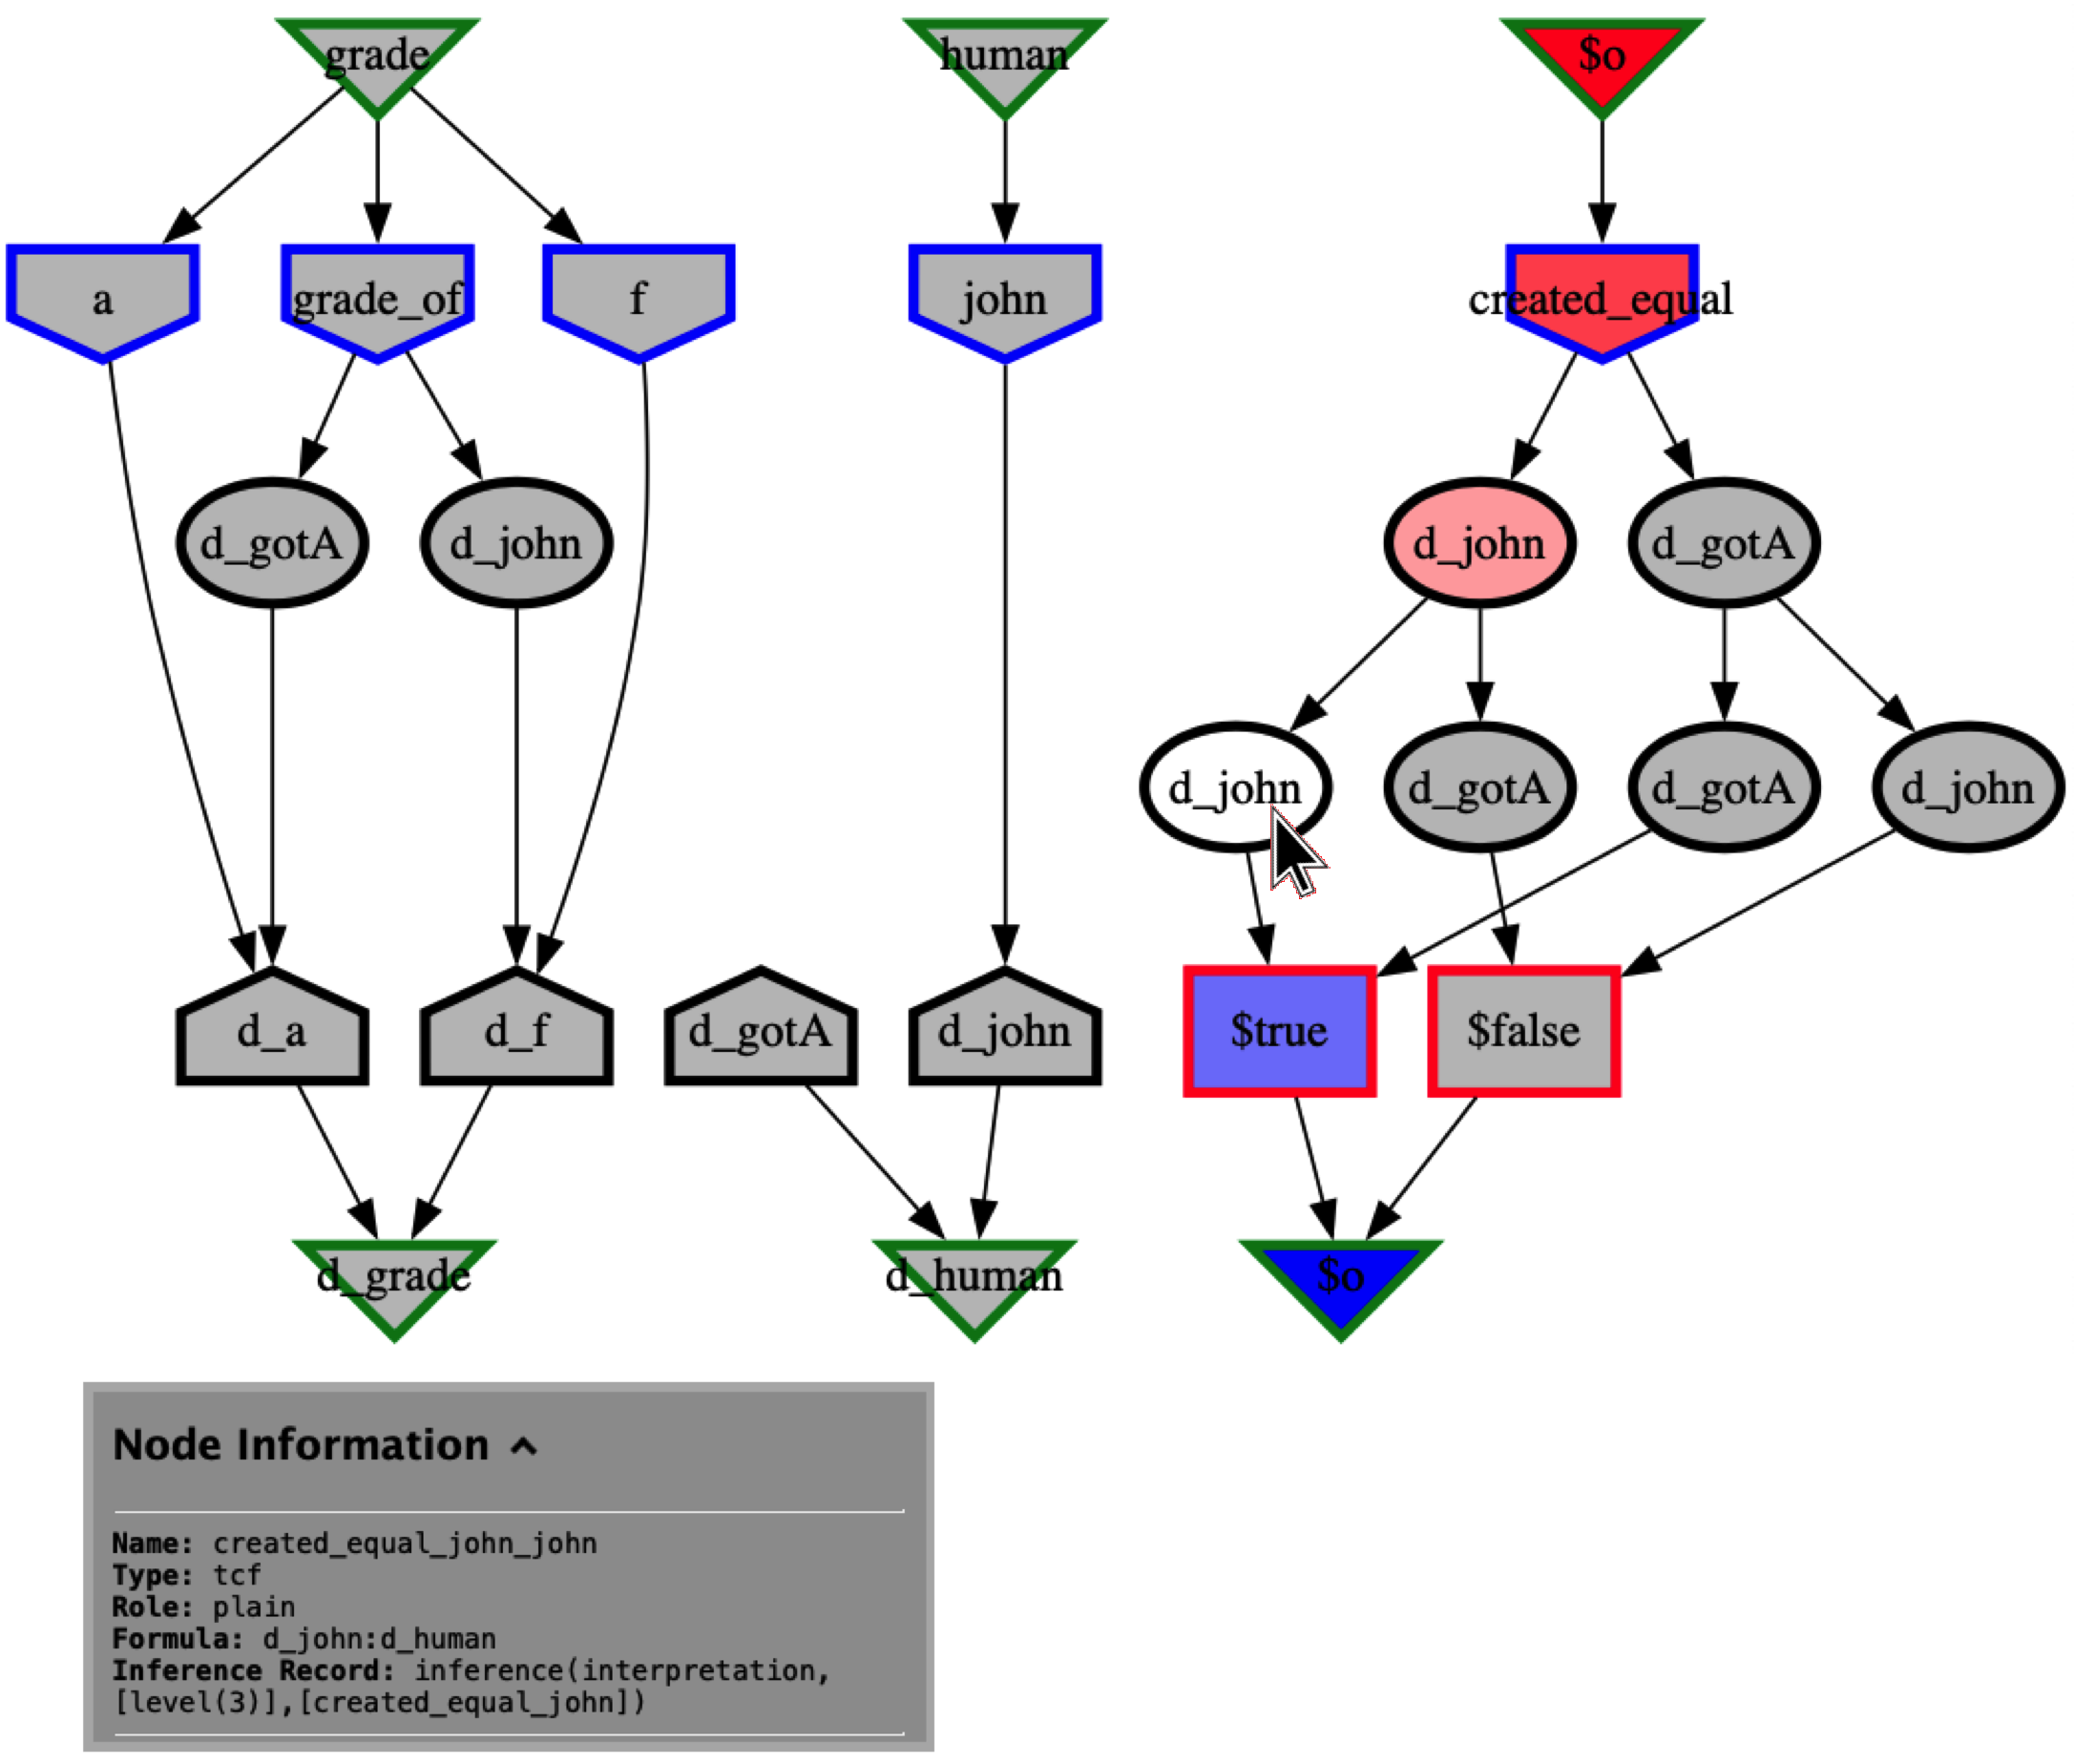
\includegraphics[width=\columnwidth]{TFF_Finite.s.IIV.pdf}
\caption{Visualization of the interpretation in Figure~\ref{TF0FiniteInterpretation}}
\label{TF0FiniteIIV}
\end{figure}

\begin{figure}[htbp]
\centering
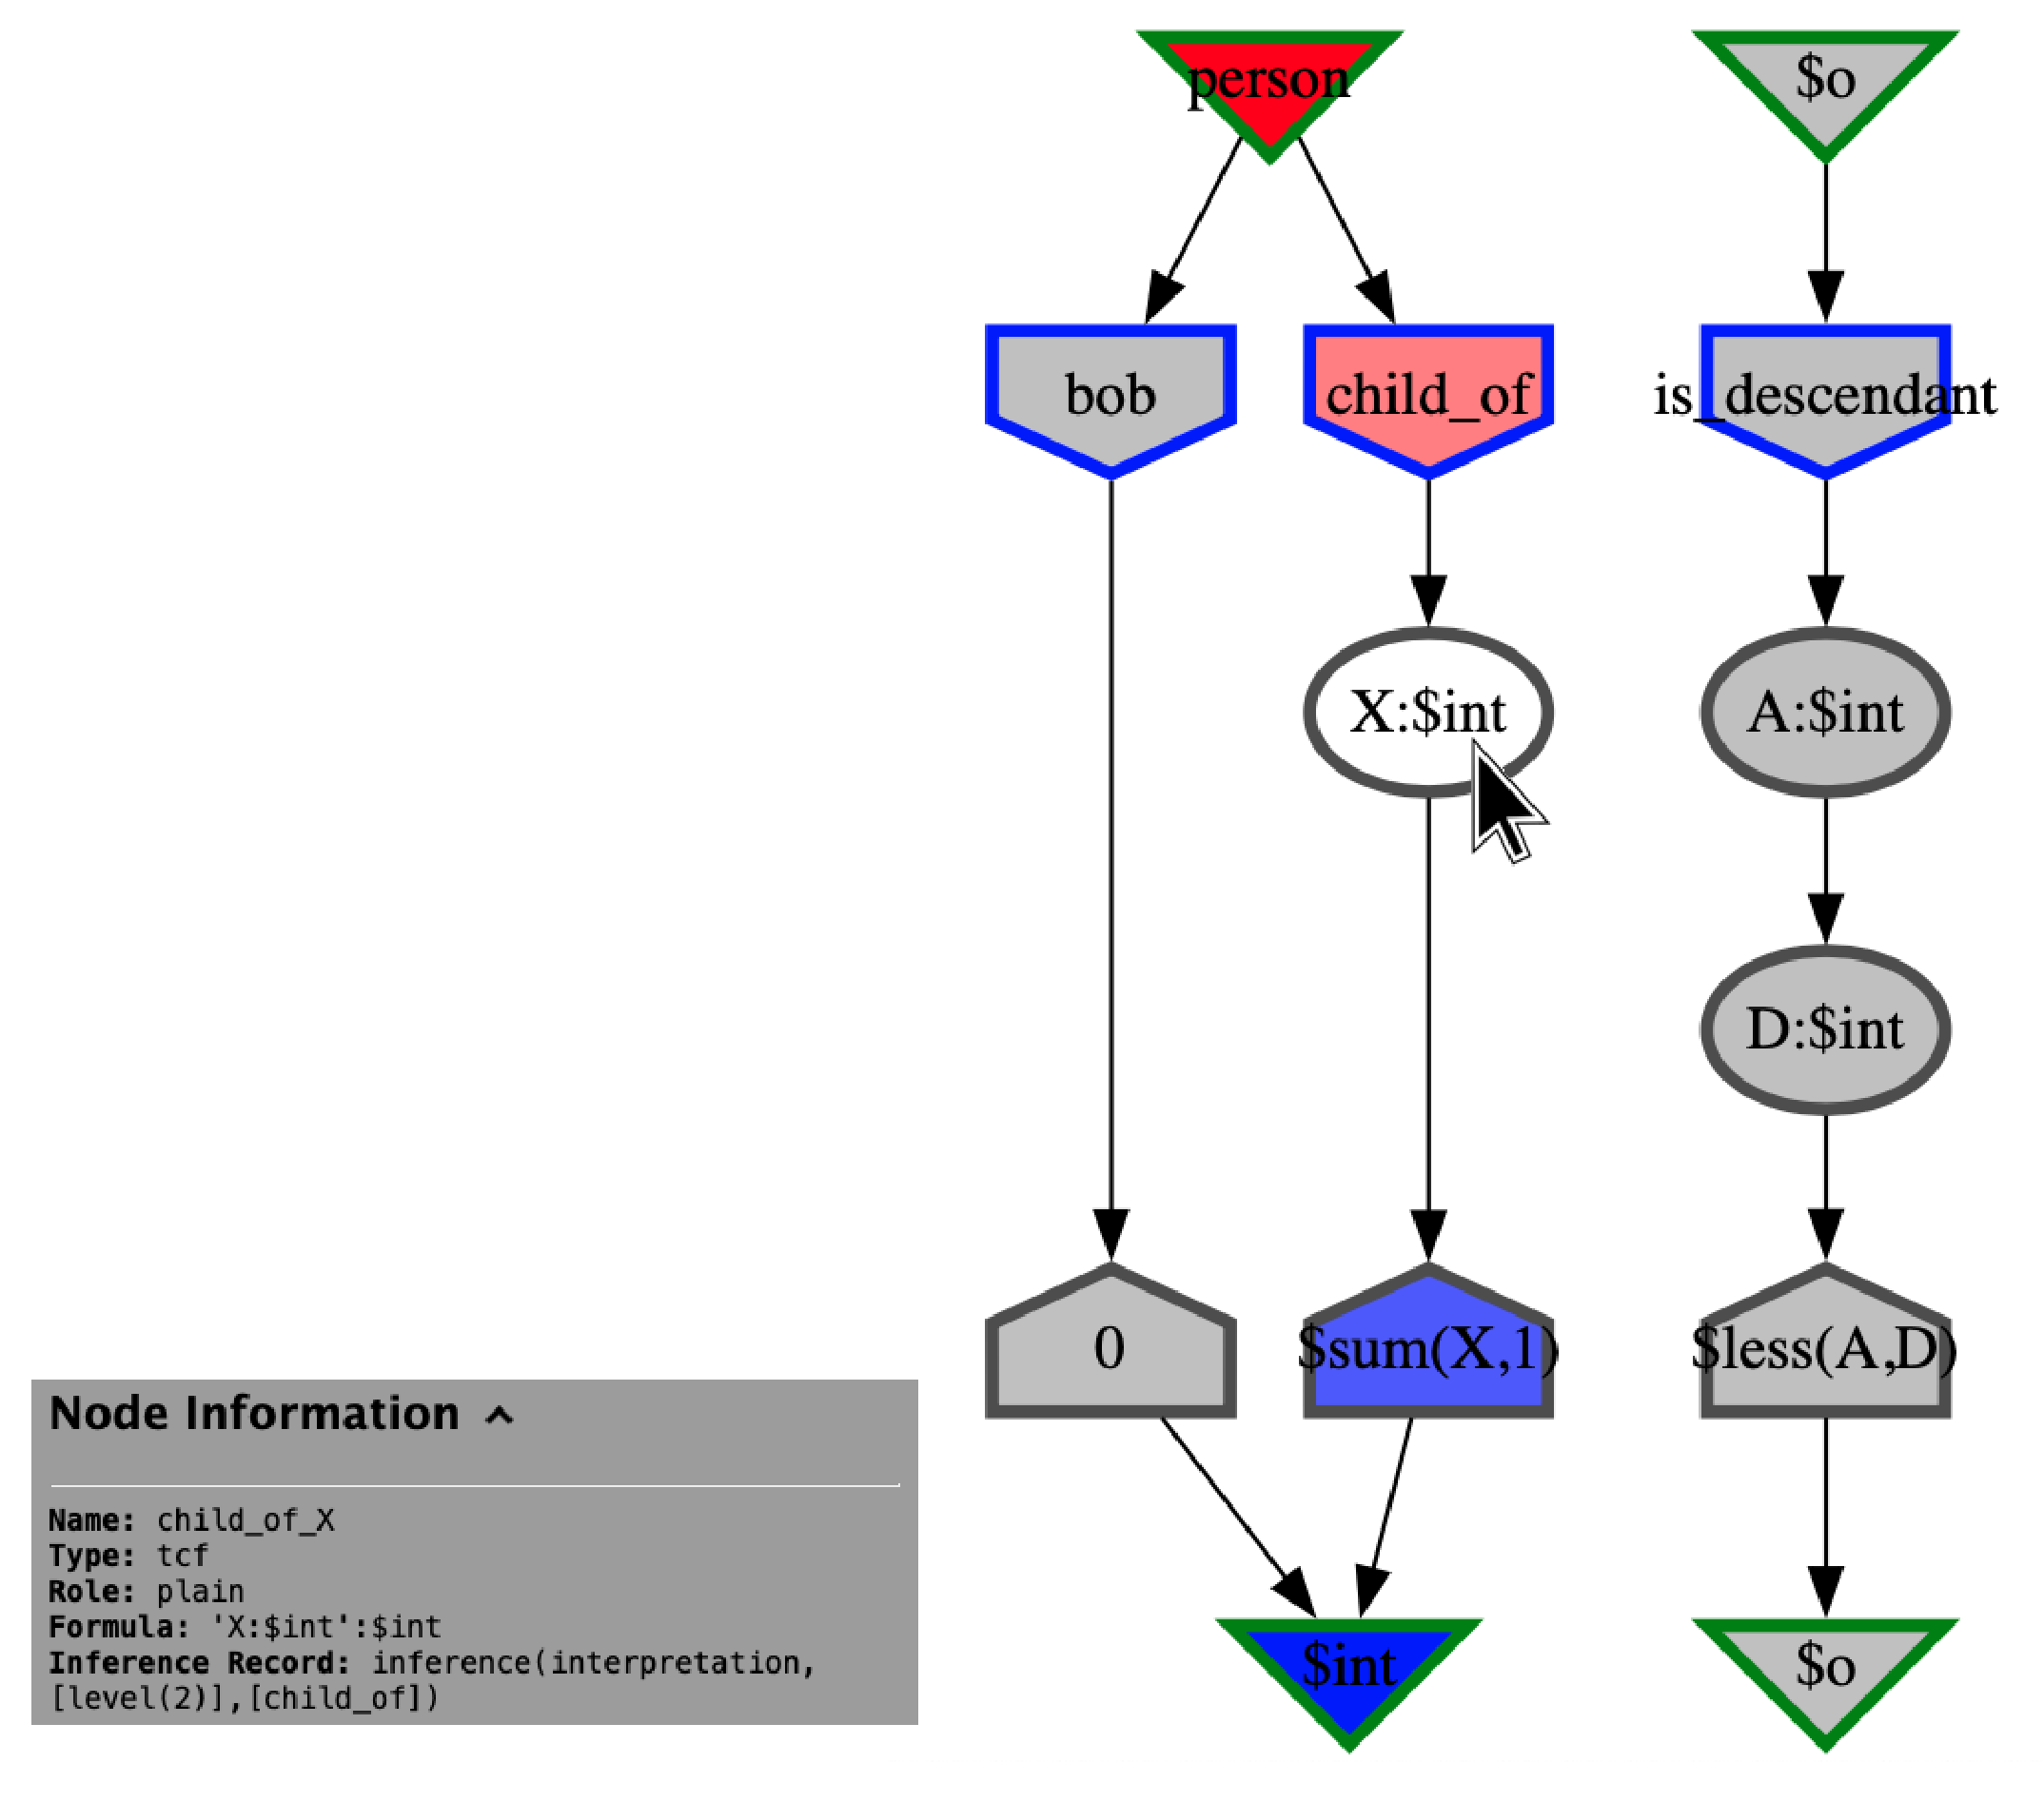
\includegraphics[width=0.45\columnwidth]{TFF_Integer.s.IIV.pdf}
\caption{Visualization of the interpretation in Figure~\ref{TF0InfiniteInterpretation}}
\label{TF0InfiniteIIV}
\end{figure}

Further inspiration might lead to improvements to these visualizations, especially for more
complex infinite interpretations.

%--------------------------------------------------------------------------------------------------
\section{Conclusion}
\label{Conclusion}

This paper describes the new TPTP format for representing Tarskian-style interpretations for
formula in typed first-order logic, using the TPTP TF0 language.
It goes on to describe a technique and implemented tool for verifying models using this 
representation, and a tool for visualizing interpretations.
The research contributes to the advancement of automated reasoning technology for model finding, 
which has several applications, including verification.

Currently this work is being extended to Kripke interpretations for formula in non-classical 
typed first-order logic \cite{SF+22}, using the TPTP TX0 language \cite{Sut22-IGPL}.
The tool to translate interpretation formulae to the format required for input to the IIV tool is 
being extended to infinite interpretations and untyped first-order interpretations.

%--------------------------------------------------------------------------------------------------
\bibliographystyle{flairs}
\bibliography{Bibliography.bib}
%--------------------------------------------------------------------------------------------------
\end{document}
%--------------------------------------------------------------------------------------------------
%% \section{Formatting Requirements in Brief}
%% We need source and PDF files that can be used in a variety of ways and can be output on a variety of devices. FLAIRS imposes some requirements on your source and PDF files that must be followed. Most of these requirements are based on our efforts to standardize conference manuscript properties and layout. These requirements are as follows, and all papers submitted to FLAIRS for publication must comply:
%% 
%% \begin{itemize}
%% \item Your .tex file must compile in PDF\LaTeX{} --- \textbf{ no .ps or .eps figure files.}
%% \item All fonts must be embedded in the PDF file --- \textbf{ this includes your figures.}
%% \item Modifications to the style sheet (or your document) in an effort to avoid extra page  are NOT allowed.
%% \item No type 3 fonts may be used (even in illustrations).
%% \item Your title must follow US capitalization rules.
%% \item \LaTeX{} documents must use the Times or Nimbus font package (do not use Computer Modern for the text of your paper).
%% \item Fonts that require non-English language support (CID and Identity-H) must be converted to outlines or removed from the document (even if they are in a graphics file embedded in the document). 
%% \item Two-column format is required for all papers.
%% \item The paper size for final submission must be US letter. No exceptions.
%% \item The source file must exactly match the PDF.
%% \item The document margins must be as specified in the formatting instructions.
%% \item The number of pages and the file size must be as specified for your event.
%% \item No document may be password protected.
%% \item Neither the PDFs nor the source may contain any embedded links or bookmarks.
%% \item Your source and PDF must not have any page numbers, footers, or headers.
%% \item Your PDF must be compatible with Acrobat 5 or higher.
%% \item Your \LaTeX{} source file (excluding references) must consist of a \textbf{single} file (use of the ``input" command is not allowed.
%% \item Your graphics must be sized appropriately outside of \LaTeX{} (do not use the ``clip" command) .
%% \end{itemize}
%% 
%% If you do not follow the above requirements, it is likely that we will be unable to publish your paper.
%% 
%% \section{What Files to Submit}
%% You must submit the following items to ensure that your paper is published:
%% \begin{itemize}
%% \item A fully-compliant PDF file.
%% \item Your  \LaTeX{}  source file submitted as a \textbf{single} .tex file (do not use the ``input" command to include sections of your paper --- every section must be in the single source file). The only exception is the bibliography, which you may include separately. Your source must compile on our system, which includes the standard \LaTeX{} support files.
%% \item All your graphics files.
%% \item The \LaTeX{}-generated files (e.g. .aux and .bib file, etc.) for your compiled source.
%% \item All the nonstandard style files (ones not commonly found in standard \LaTeX{} installations) used in your document (including, for example, old algorithm style files). If in doubt, include it.
%% \end{itemize}
%% 
%% Your \LaTeX{} source will be reviewed and recompiled on our system (if it does not compile, you may incur late fees).   \textbf{Do not submit your source in multiple text files.} Your single \LaTeX{} source file must include all your text, your bibliography (formatted using flairs.bst), and any custom macros. Accompanying this source file, you must also supply any nonstandard (or older) referenced style files and all your referenced graphics files. 
%% 
%% Your files should work without any supporting files (other than the program itself) on any computer with a standard \LaTeX{} distribution. Place your PDF and source files in a single tar, zipped, gzipped, stuffed, or compressed archive. Name your source file with your last (family) name.
%% 
%% \textbf{Do not send files that are not actually used in the paper.} We don't want you to send us any files not needed for compiling your paper, including, for example, this instructions file, unused graphics files, and so forth.  
%% 
%% \section{Using \LaTeX{} to Format Your Paper}
%% 
%% The latest version of the FLAIRS style file is available on FLAIRS's website. Download this file and place it in a file named ``flairs.sty" in the \TeX\ search path. Placing it in the same directory as the paper should also work. You must download the latest version.
%% 
%% The following packages are incompatible with flairs.sty and/or flairs.bst and must not be used (this list is not exhaustive --- there are others as well):
%% \begin{itemize}
%% \item hyperref
%% \item natbib
%% \item geometry
%% \item titlesec
%% \item layout
%% \item caption
%% \item titlesec
%% \item T1 fontenc package (install the CM super fonts package instead)
%% \end{itemize}
%% 
%% \subsection{Illegal Commands}
%% The following commands may not be used in your paper:
%% \begin{itemize}
%% \item \textbackslash input
%% \item \textbackslash vspace (when used before or after a section or subsection)
%% \item \textbackslash addtolength 
%% \item \textbackslash columnsep
%% \item \textbackslash top margin (or text height or addsidemargin or even side margin)
%% \end{itemize}
%% 
%% \subsection{Paper Size, Margins, and Column Width}
%% Papers must be formatted to print in two-column format on 8.5 x 11 inch US letter-sized paper. The margins must be exactly as follows: 
%% \begin{itemize}
%% \item Top margin: .75 inches
%% \item Left margin: .75 inches
%% \item Right margin: .75 inches
%% \item Bottom margin: 1.25 inches
%% \end{itemize} 
%% 
%% 
%% The default paper size in most installations of \LaTeX{} is A4. However, because we require that your electronic paper be formatted in US letter size, you will need to alter the default for this paper to US letter size. Assuming you are using the 2e version of \LaTeX{}, you can do this by including the [letterpaper] option at the beginning of your file: 
%% \textbackslash documentclass[letterpaper]{article}. 
%% 
%% This command is usually sufficient to change the format. Sometimes, however, it may not work. Use PDF\LaTeX{} and include
%% \textbackslash setlength\{\textbackslash pdfpagewidth\}\{8.5in\}
%% \textbackslash setlength\{\textbackslash pdfpageheight\}\{11in\}
%% in your preamble. 
%% 
%% \textbf{Do not use the Geometry package to alter the page size.} Use of this style file alters flairs.sty and will result in your paper being rejected. 
%% 
%% 
%% \subsubsection{Column Width and Margins.}
%% To ensure maximum readability, your paper must include two columns. Each column should be 3.3 inches wide (slightly more than 3.25 inches), with a .375 inch (.952 cm) gutter of white space between the two columns. The flairs.sty file will automatically create these columns for you. 
%% 
%% \subsection{Overlength Papers}
%% If your paper is too long, turn on \textbackslash frenchspacing, which will reduce the space after periods. Next,  shrink the size of your graphics. Use \textbackslash centering instead of \textbackslash begin\{center\} in your figure environment. If these two methods don't work, you may minimally use the following. For floats (tables and figures), you may minimally reduce \textbackslash floatsep, \textbackslash textfloatsep, \textbackslash abovecaptionskip, and \textbackslash belowcaptionskip. For mathematical environments, you may minimally reduce \textbackslash abovedisplayskip, \textbackslash belowdisplayskip, and \textbackslash arraycolsep. You may also alter the size of your bibliography by inserting \textbackslash fontsize\{9.5pt\}\{10.5pt\} \textbackslash selectfont
%% right before the bibliography. 
%% 
%% Commands that alter page layout are forbidden. These include \textbackslash columnsep, \textbackslash topmargin, \textbackslash topskip, \textbackslash textheight, \textbackslash textwidth, \textbackslash oddsidemargin, and \textbackslash evensizemargin (this list is not exhaustive). If you alter page layout, you will be required to pay the page fee \textit{plus} a reformatting fee. Other commands that are questionable and may cause your paper to be rejected include  \textbackslash parindent, and \textbackslash parskip. Commands that alter the space between sections are also questionable. The title sec package is not allowed. Regardless of the above, if your paper is obviously ``squeezed" it is not going to to be accepted. Before using every trick you know to make your paper a certain length, try reducing the size of your graphics or cutting text instead.
%% 
%% \subsection{Credits}
%% Any credits to a sponsoring agency should appear in the acknowledgments section, unless the agency requires different placement. If it is necessary to include this information on the front page, use
%% \textbackslash thanks in either the \textbackslash author or \textbackslash title commands.
%% For example:
%% \begin{quote}
%% \begin{small}
%% \textbackslash title\{Very Important Results in AI\textbackslash thanks\{This work is
%%  supported by everybody.\}\}
%% \end{small}
%% \end{quote}
%% Multiple \textbackslash thanks commands can be given. Each will result in a separate footnote indication in the author or title with the corresponding text at the botton of the first column of the document. Note that the \textbackslash thanks command is fragile. You will need to use \textbackslash protect.
%% 
%% Please do not include \textbackslash pubnote commands in your document.
%% 
